\documentclass[professionalfonts, xcolor={usenames,svgnames,x11names,table}]{beamer}

\usetheme{SBU}
\usepackage[charter]{mathdesign}
\usepackage[scaled]{helvet}

\usepackage{mypackages}
\usepackage{mycommands}
\newcommand{\subpoint}[1]{{small\color{LightSteelBlue4}#1}}
% \renewcommand{\treeload}[1]{} % uncomment to prevent trees from loading
                                % --> faster compilation

\definecolor{mygray}{gray}{0.9}
\definecolor{cadmiumgreen}{rgb}{0.0, 0.42, 0.24}
\definecolor{teagreen}{rgb}{0.82, 0.94, 0.75}

\usepackage{forest}
\useforestlibrary{linguistics}
\forestapplylibrarydefaults{linguistics}
\usepackage{gb4e}

\usepackage{tikz}
\usepackage{tikz-qtree}
\usetikzlibrary{automata, calc, positioning}

\title[TSL]{%
    \texorpdfstring{Tier-Based Strictly Local Analyses\\of Negation in Mandarin Chinese}%
    {Tier-Based Strictly Local Analyses of Negation in Mandarin Chinese}}
\author{%
    Hongchen Wu
}

\institute{Stony Brook University\\hongchen.wu@stonybrook.edu}
\date{Computational Phonology Workshop 2016\\Dec. 12, 2016}


\begin{document}
\unnumbered{
\begin{frame}
	\titlepage
\end{frame}
}

\unnumbered{
\begin{frame}{Take Home Message}
    \begin{block}{Result\ldots}
        The locality of co-occurrence of Mandarin Chinese negation markers (\textit{bu} and \textit{mei}) can be captured by a Tier Based-Strictly Local (TSL) grammar.
    \end{block}

    \pause
    \begin{alertblock}{\ldots supports TSL trend!}
        TSL can capture properties of syntactic domains beyond move and merge dependencies
           
    \end{alertblock}
\end{frame}
}

\unnumbered{
\begin{frame}{Outline}
   \tableofcontents
\end{frame}
}

\section[Overview]{Overview}

\begin{frame}{TSL trend}
 \begin{block}{TSL across language modules}
    \vspace{.8em}
        \begin{tabular}{cccc}
            & Complexity & Data Structure & Related Paper(s)\\[1.5ex]
            
             Phonology & TSL & strings & Heinz (2015)\\[1.5ex]
             
             Morphology & TSL & strings & Aks\"{e}nova et al. (2016) \\[1.5ex]
             \pause
             
            
            \highlight{Syntax} & \highlight{TSL} & \highlight{trees} & Graf (2016)\\
        \end{tabular}    


 \end{block}

   
    \uncover<3>{
      \vspace{2em}
             \colorbox{cadmiumgreen}{\textcolor{white}{TSL syntax: ``Hard to say in full generality, but Merge and Move are TSL.}}
     }
\end{frame}


\begin{frame}{TSL syntax}
Tree $n$-gram grammars: 
    \begin{itemize}
        \item All patterns are described by forbidden \textit{n}-gram(s).
        \item A derivational tree is well formed iff no tier \textit{T} contains any forbidden \textit{n}-gram(s).
    \end{itemize}
  %
  \pause
    \begin{exampleblock}{Example: TSL operating over trees}
        \centering
        
\begin{tabular}{lrl}
\begin{tabular}{l}
              \only<-2>{\scalebox{0.85}{ \begin{forest}
 for tree={parent anchor=south, child anchor=north}
   [,phantom,{l=0}
         [S,name=s
           [NP,name=np1
               [John]
               ]
           [VP
               [V
                   [likes]
               ]
               [NP,name=np2
                   [Mary]
               ]
           ]
       ]  
   ]
\end{forest}}}
 \end{tabular}
&
 \begin{tabular}{l}   
 \pause 
             \scalebox{0.85}{\begin{forest}
 for tree={parent anchor=south, child anchor=north}
   [,phantom,{l=0}
         [S,blue,name=s
           [NP,blue,name=np1
               [John]
               ]
           [VP
               [V
                   [likes]
               ]
               [NP,blue,name=np2
                   [Mary]
               ]
           ]
       ]  
       [S,draw,blue,name=ts
           [NP,draw,blue,name=tnp1]
           [NP,draw,blue,name=tnp2]
       ]
   ]
   %
   \foreach \Node in {s,np1,np2}
       \draw[dashed,gray,opacity=.99] (\Node) to (t\Node);
\end{forest}} 
 \end{tabular}\hspace{8mm}
 &
 \begin{tabular}{l} 
 \pause
\only<-4>{\textcolor{purple}{*}\scalebox{0.9}{\begin{forest}
for tree={edge={dashed, purple}, purple}
 [S [$>3$ NP,roof]]
\end{forest}}}\\
%
\pause
\textcolor{red}{*}\scalebox{0.9}{\begin{forest}
for tree={edge={dashed,red}, red}
 [S [$<3$ NP,roof]]
\end{forest}}
\end{tabular}
            \end{tabular}   
    \end{exampleblock}
\end{frame}



\section[TSL analyses]{TSL analyses}

\begin{frame}{Negation in Mandarin}

 \begin{itemize}
        \item \textit{bu} (`Neg1') and \textit{mei} (`Neg2')      
    \end{itemize}
    
\begin{exampleblock}{Examples: possible negation maker combinations}
\pause
 \begin{exe}
 \ex\label{mylabel} \gll Ni  \textcolor{blue}{bu}  neng  \textcolor{blue}{bu}  gongzuo. \\
                     you  Neg1  can  Neg1  work \\
                \glt `You  can't not work.'
    \pause

     \ex \gll Ni  \textcolor{blue}{bu}  neng  \textcolor{blue}{mei}  you gongzuo. \\
                     you  Neg1  can  Neg1  have  job \\
                \glt `You can't not have a job.' 
\end{exe} 
\pause
\begin{itemize}
\item \textcolor{cadmiumgreen}{For any sentence, negation markers do not need to be the same. }
\end{itemize}  
\end{exampleblock}

\end{frame}
%wo bu neng bu he jiu
%wo mei neng bu he jiu
%wo mei  bu he jiu.
%wo mei mei he jiu.

\begin{frame}{Negation in Mandarin}

 \begin{itemize}
        \item \textit{bu} (`Neg1') and \textit{mei} (`Neg2')      
    \end{itemize}
    
\begin{exampleblock}{Examples: possible negation maker combinations}
\pause
 \begin{exe}
   \ex \gll Wo  \textcolor{blue}{mei}  \textcolor{blue}{bu}  chi  zaofan. \\
                     I  Neg2  Neg1  eat  breakfast \\
                \glt `It's not the case that I don't eat breakfast.'
    \pause

     \ex \gll Wo  \textcolor{blue}{mei}  changchang  \textcolor{blue}{bu}  chi  zaofan. \\
                     I  Neg2  often  Neg1  eat  breakfast \\
                \glt `It's not the case that I often don't eat breakfast.' 
\end{exe} 
\pause
\begin{itemize}
\item \textcolor{cadmiumgreen}{Sentences with negation markers being adjacent are well-formed, as are sentences with non-adjacent negation markers. Hence the restrictions on co-occurance of Neg1 and Neg2 are not about adjacency.}
\end{itemize}  
\end{exampleblock}
\end{frame}


\begin{frame}{A TSL grammar}
 \begin{block}{Requirement:}
        There must be \textcolor{blue}{at least one TP} in between any two negation markers.
    \end{block}
  \vspace{1em}
  
  \begin{columns}

\column{.31\linewidth}
\pause
\begin{exampleblock}{Tiers and tree $n$-gram}
 \centering
    Tier: TP, Neg\\\vspace{1em}
%
        \textcolor{red}{*}\begin{forest}
for tree={edge={dashed,red},red}
 [TP[$>1$ Neg,roof]]
\end{forest}
\end{exampleblock}

\column{.4\linewidth}
\centering
\pause
\begin{tabular}{ll}
\begin{tabular}{l}
 \only<-3>{\input{./code/2.tikz}}
 \end{tabular}
 &
\begin{tabular}{l}
\pause 
 \begin{forest}
for tree={parent anchor=south, child anchor=north,l+=5mm}
[TP,blue
[Neg,blue][TP,blue[Neg,blue,roof]]]
\end{forest}
 \end{tabular}
 
\end{tabular}

\end{columns}
 \end{frame}
 
 
\begin{frame}{Example of Ill-Formed Derivation}
\begin{columns}
\column{.585\linewidth}
 \begin{exe}
\ex \gll $^*$Wo  \textcolor{blue}{mei}  \textcolor{blue}{mei}  chi  zaofan. \\
                    \textcolor{white}{$^*$}I  Neg2  Neg2  eat  breakfast \\
                \glt \textcolor{white}{$^*$}`(lit.) It's not the case that I didn't eat breakfast.'
\end{exe}
  \vspace{2em}  
%
\pause
\begin{tabular}{ll}
\centering
\hspace{2mm}
\begin{tabular}{l}
\visible<4->{\textcolor{cadmiumgreen}{Tree $n$-gram}\\
        \colorbox{mygray}{\textcolor{red}{*}\begin{forest}
for tree={edge={dashed,red},red}
 [TP[$>1$ Neg,roof]]
\end{forest}}}
\end{tabular}\hspace{3mm}
&
\begin{tabular}{l}
\visible<3->{*\begin{forest}
for tree={parent anchor=south, child anchor=north}
[TP,red[Neg,red][Neg,red]]
            \end{forest}}
 \end{tabular}
 \end{tabular}

\column{.415\linewidth}
 \visible<2->{\scalebox{0.8}{
\begin{forest}
 for tree={s sep=(5.5-level)*2mm, parent anchor=south, child anchor=north}
   [,phantom,{l=-1mm}
       [TP,blue,draw
           [wo]
               [NegP
                   [Neg,blue,draw
                     [mei]]
                   [NegP
                     [Neg,blue,draw
                       [mei]]
                          [VP[chi \ zaofan,roof]
                          ]
                    ]
                ]
          ]
    ]                    
\end{forest}}}

\end{columns}
\end{frame} 
 
 \begin{frame}{Example of Well-Formed Derivation}
\begin{columns}
\column{.585\linewidth}
 \begin{exe}
\exr{mylabel} \gll Ni  \textcolor{blue}{bu}  neng  \textcolor{blue}{bu}  gongzuo. \\
                     you  Neg1  can  Neg1  work \\
                \glt `You  can't not work.'
\end{exe}
  \vspace{2em}  
\pause

\begin{tabular}{ll}
\centering
\hspace{5mm}
\begin{tabular}{l}
\visible<4->{\textcolor{cadmiumgreen}{Tree $n$-gram}\\
        \colorbox{mygray}{\textcolor{red}{*}\begin{forest}
for tree={edge={dashed,red},red}
 [TP[$>1$ Neg,roof]]
\end{forest}}}
\end{tabular}\hspace{6mm}
&
\begin{tabular}{l}
\visible<3->{\begin{forest}
 [TP,blue,name=ttp1
           [Neg,blue,name=tneg1]
           [TP,blue,name=ttp2
               [Neg,blue,name=tneg2]
           ]
      ]
 \end{forest}}
 \end{tabular}
 \end{tabular}


\column{.415\linewidth}
 \visible<2->{\scalebox{0.8}{
\begin{forest}
 for tree={s sep=(5.5-level)*2mm, parent anchor=south, child anchor=north}
   [,phantom,{l=-1mm}
       [TP,blue,draw,name=tp1
           [ni]
               [NegP
                   [Neg,blue,draw,name=neg1
                     [bu]]
                  [AuxP
                   [neng]
                     [\dots
                        [\dots]
                      [TP,blue,draw,name=tp2
                          [\dots]
                          [NegP
                            [Neg,blue,draw,name=neg2 
                              [bu]]
                            [VP[gongzuo,roof]]]]]]]]
      ]
\end{forest}}}

\end{columns}
\end{frame}
 
 \section[Problematic cases]{Problematic cases}
 
 \begin{frame}{AP on the tier?}
\begin{exe}
\ex \label{mylabel1}\gll Wo  bu  mai  \textcolor{red}{mei}  yiyi  \textcolor{blue}{bu}  haokan  de  hua. \\
                     I  Neg1  buy  Neg2  meaning  Neg1  beautiful  DE  painting \\
                \glt `I do not buy paintings that are not meaningful nor beautiful.'
\end{exe}

\pause
\begin{columns}
\column{.3\linewidth}
\scalebox{0.8}{\begin{forest}
 for tree={s sep=(5.5-level)*2mm, parent anchor=south, child anchor=north}
   [,phantom,{l=-3mm}
       [TP,blue,draw
           [wo]
               [NegP
                   [Neg,blue,draw
                     [bu]]
                   [vP
                      [v
                         [mai]]
                      [\dots
                         [\textcolor{blue}{Neg1} \  \textcolor{blue}{Neg2},roof]]]]]]
 \end{forest}}

\pause
\column{.5\linewidth}
Possible solution:\\
\begin{itemize}
\item Putting AP on the tier: \\treating the two constituents \textit{mei yiyi} (`not meaningful') and \textit{bu haokan} (`not beautiful') as coordinate APs. 
\end{itemize}

\end{columns}
\end{frame}


 \begin{frame}{AP on the tier?}
\textcolor{cadmiumgreen}{However, the two constituents \textit{mei yiyi} (`not meaningful') and \textit{bu haokan} (`not beautiful') are different from normal APs. }
%because they do not show scope relations.
\begin{exe}
\exr{mylabel1}\gll Wo  \textcolor{blue}{bu}  mai  \textcolor{red}{mei}  yiyi  \textcolor{blue}{bu}  haokan  de  hua. \\
                     I  Neg1  buy  Neg2  meaning  Neg1  beautiful  DE  painting \\
                \glt `I do not buy paintings that are not meaningful nor beautiful.'
 \pause               
\ex \gll Wo  bu  mai  \textcolor{blue}{bu}  haokan  \textcolor{red}{mei}  yiyi  de  hua. \\
                     I  Neg1  buy  Neg1  beautiful  Neg2  meaning  DE  painting \\
                \glt `I do not buy paintings that are not meaningful nor beautiful.'
\pause

\ex
\begin{xlist}
\ex \gll yige  xiao  de  gui  de  fangzi \\
            a-CL  small  DE  expensive  DE  house \\
                \glt `a small expensive house'
  
\ex \gll yige  gui  de  xiao  de  fangzi \\
            a-CL  expensive  DE  small  DE  house \\
                \glt `a expensive small house'
\end{xlist}                
\end{exe}

\end{frame}

 
  \begin{frame}{AP on the tier?}
Another Possible solution:\\
\begin{itemize}
\item Analyzing as relative clauses (a.k.a, two CPs) : \\treating the two constituents \textit{mei yiyi} (`not meaningful') and \textit{bu haokan} (`not beautiful') as two relative clauses modifying the head noun \textit{hua} (`paintings') together. \\
In this way, inside the syntactic structure of (6), there are two TPs in between the two negation markers.\\
With this analysis, we only need TP on the tier for this moment. 
\end{itemize}
\pause

\begin{alertblock}{These two solutions...}
\begin{itemize}
\item Either one could work. 
\item Both of them can be handled by TSL!
\end{itemize}
\end{alertblock}
 \end{frame}
 
  
 \begin{frame}{VP on the tier?}
\begin{exe}
  \ex \gll Ta \textcolor{blue}{mei} kan \textcolor{blue}{bu} dong zhe-ben shu. \\
                       wo  Neg2  read  Neg1  understand  this-CL  book \\
                \glt `It's not the case the I can read and not understand this book.'
\end{exe}

%\pause
%\begin{itemize}
%\item The postverbal predicative complement \textit{bu dong} (`not understand')  is rather an infinitive clause (a.k.a, TP) than a PP adjunction. 

\pause
\begin{columns}
\column{.3\linewidth}
\scalebox{0.8}{\begin{forest}
 for tree={s sep=(5.5-level)*2mm, parent anchor=south, child anchor=north}
   [,phantom,{l=-3mm}
       [TP,blue,draw
           [wo]
               [NegP
                   [Neg,blue,draw
                     [mei]]
                   [VP
                      [V 
                         [kan \ \textcolor{blue}{Neg} \ dong,roof]]
                      [NP
                         [na\ ben\ shu,roof]]]]]]
 \end{forest}}
 
 \pause
\column{.5\linewidth}
Possible solution:\\
\begin{itemize}
\item Putting VP on the tier: \\treating the constituent \textit{kan bu dong} (`can read and not understand') as a complex V compound, like the way most linguists treat V-\textit{de}-postverbal complement construction. (Zhuang $\&$ Liu 2011)
\end{itemize}
\end{columns}
\end{frame}
  
  
  \begin{frame}{VP on the tier?}
  
\textcolor{cadmiumgreen}{However, treating verb and its postverbal predicative complement as a complex V compound may have some downsides.}


\begin{itemize}
\pause
\item Neg is not a head in this case.
\pause
\item Putting VP on the tier makes this TSL grammar more restricted, which might block some well-formed sentences.  

\end{itemize}

\pause
\textcolor{cadmiumgreen}{Meanwhile, for postverbal predicate complement, the structure is rich enough to be clausal, for example, to get an infinite TP clause.} \\
\pause
\begin{exe}
\ex \gll wo  wan  DE  \textcolor{blue}{bu}  \textcolor{blue}{xiang}  \textcolor{blue}{shangxue}   \textcolor{blue}{le}. \\
            I  play  DE  Neg  want  go-to-school  ASP. \\
                \glt `(lit.) I played so much that I do not want to go to school any more.'
\end{exe}

\end{frame}




  \begin{frame}{VP on the tier?}
Another Possible solution:\\
\begin{itemize}
\item Analyzing the postverbal predicative complement \textit{bu dong} (`not understand')  as an infinitive clause (a.k.a, TP). \\
With this analysis, we only need TP on the tier for this moment. 
\end{itemize}
\pause

\begin{alertblock}{These two solutions...}
\begin{itemize}
\item Either one could work. 
\item Both of them can be handled by TSL!
\end{itemize}
\end{alertblock}
 \end{frame}

  
\begin{frame}{Beyond TSL?}
\begin{alertblock}{Two kinds of localities that can not be handled by TSL...}
\begin{itemize}
\item Sibling dependency
\item C-command relation
\end{itemize}
\end{alertblock}
 
 \pause
    \begin{exampleblock}{Examples}
        \centering
        
\begin{tabular}{ll}
\begin{tabular}{l}
              \only<-2>{\scalebox{0.9}{ \begin{forest}
 for tree={parent anchor=south, child anchor=north}
  [,phantom,{l=0}
         [X,blue,name=x
           [Y,blue,name=y]
           [\dots
               [\dots]
                   [Z,blue,name=z]
          ]]
       [X,draw,blue,name=tx
           [Y,draw,blue,name=ty]
           [Z,draw,blue,name=tz]
       ]
   ]
   %
   \foreach \Node in {x,y,z}
       \draw[dashed,red,opacity=.99] (\Node) to (t\Node);
\end{forest}}}
 \end{tabular}
&
 \begin{tabular}{l}
              \only<3->{\scalebox{0.85}{ \begin{forest}
 for tree={parent anchor=south, child anchor=north}
  [,phantom,{l=0}
         [A,blue,name=a
           [B,blue,name=b]
           [\dots
               [C]
                   [D,blue,name=d]
          ]]
       [A,draw,blue,name=ta
           [B,draw,blue,name=tb]
           [D,draw,blue,name=td]
       ]
   ]
   %
   \foreach \Node in {a,b,d}
       \draw[dashed,red,opacity=.99] (\Node) to (t\Node);
\end{forest}}}
 \end{tabular}
            \end{tabular}   
    \end{exampleblock}

\end{frame}

\begin{frame}{Sibling Dependency?}

 \begin{exe}
        \ex
        \begin{xlist}
            \ex \label{mylabel2} \gll Wo  \textcolor{blue}{mei}  \textcolor{blue}{bu}  kaixin. \\
                     I  Neg2  Neg1  happy \\
                \glt `It's not the case that I'm not happy.'
             \pause
             \ex \gll Wo  \textcolor{blue}{mei}  hen  \textcolor{blue}{bu}  kaixin. \\
                     I  Neg2  very  Neg1  happy \\
                \glt `It's not the case that I'm very unhappy.
                \pause
            \ex \gll Wo  \textcolor{blue}{mei}  \textcolor{blue}{bu}  kaixin,  ta  ye  \textcolor{blue}{mei}. \\
                     I  Neg2  Neg1  happy, he  too  Neg2 \\
                \glt `It's not the case that I'm not happy. Also, It's not the case that he is not happy.'
                \end{xlist}
\end{exe}

\begin{itemize}
\pause
\item \textcolor{cadmiumgreen}{Neg1 and Neg2 are not real siblings!} 
\end{itemize}
\end{frame}


\begin{frame}{Asymmetrical C-command relation matters?}
 \begin{exe}
            \exr{mylabel2} \gll Wo  \textcolor{blue}{mei}  \textcolor{blue}{bu}  kaixin. \\
                     I  Neg2  Neg1  happy \\
                \glt `It's not the case that I'm not happy.'
 \pause               
   \ex \gll Lisi  \textcolor{blue}{bu}  shi  \textcolor{blue}{mei}  mai  che. \\
                 Lisi  Neg1  be  Neg2  buy  car \\
                \glt `It's not the case that Lisi hasn't bought a car.'
\end{exe}

 \pause
    \begin{exampleblock}{Examples}
        \centering
        
\begin{tabular}{ll}
\begin{tabular}{l}
\scalebox{0.7}{
\begin{forest}
 for tree={s sep=(8-level)*2mm, parent anchor=south, child anchor=north,l-=25mm}
      [\dots
           [Neg2,blue]
               [\dots
                   [,phantom]
                  [TP,blue
                  [\textcolor{blue}{Neg1} \ kaixin,roof]]]]
    \end{forest}}  
\end{tabular}
&
\begin{tabular}{l}
\scalebox{0.7}{
\begin{forest}
 for tree={s sep=(8-level)*2mm, parent anchor=south, child anchor=north,l-=25mm}
        [\dots
           [Neg1,blue]
               [FocP
                  [shi]
                  [TP,blue
                  [\textcolor{blue}{Neg2} \ mai che,roof]]]]
    \end{forest}}
\end{tabular}
\end{tabular}
 \end{exampleblock}
\end{frame}


\section[Conclusion]{Conclusion}
\begin{frame}{Main points}
\begin{itemize}
\item The locality of co-occurrence of Mandarin Chinese negation markers is TSL bound. 
\pause
\item This shows that syntactic notion of locality domain can be captured by the class of TSL dependencies.
\item Also it provides more support  for the TSL trend across language modules
\end{itemize}  
\pause 
\begin{block}{Future research}
Investigating whether negation patterns have similar formal complexity across languages.
\end{block}
\end{frame}


\begin{frame}{Acknowledgments}
Many thanks to Thomas Graf, and my colleagues in the Computational Phonology Seminar group and in Richard Larson's advisee group. 
\end{frame}


\begin{frame}{References}
\begin{itemize}
\item \textbf{Aks\"{e}nova, Al\"{e}na}, and T. Graf, and S. Moradi. 2016. Morphotactics as tier-based strictly local dependencies. In \textit{Proceedings of the 14th Annual SIGMORPHON}.
\item \textbf{Graf, Thomas}. 2016. Computational Parallels Across Language Modules (\href{http://thomasgraf.net/doc/talks/Graf16Yaletalk.pdf}{slides available online}).
\item \textbf{Heinz, Jeffrey}. 2015. The computational nature of phonological generalizations. Ms., University of Delaware.
\end{itemize}  
\end{frame}

\begin{frame}
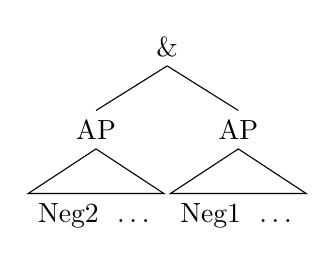
\begin{tikzpicture}
     \Tree
          [.{$\&$} [.AP  \edge[roof]; {Neg2 \ {\dots}} ][.AP  \edge[roof]; {Neg1 \ {\dots}} ]]
            \end{tikzpicture}
\end{frame}

\begin{frame}
\begin{exe}
\ex \gll Wo  kan   jufajiegou  mei  kan  bu  dong. \\
                 I  read  \textit{Syntax}  Neg2  read  Neg1  understand \\
                \glt `It's not the case that I read Syntax and not understand it.'
\end{exe}
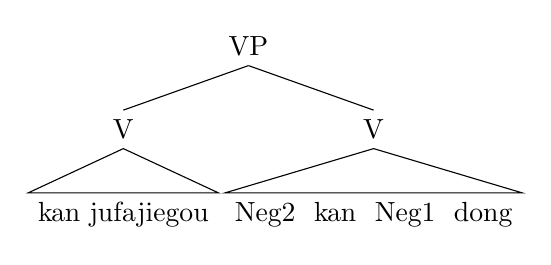
\begin{tikzpicture}
     \Tree
          [.VP [.V  \edge[roof]; {kan\ jufajiegou} ][.V  \edge[roof]; {Neg2 \ kan \ Neg1 \ dong} ]]
            \end{tikzpicture}
\end{frame}

\end{document}